\section{Learning curves}
\label{sec:appendix_curves}

Figure \ref{fig:app_plot} shows training curves for all the \textit{target} games in the Atari domain.
We plot learning curves for two column, three column and four column progressive networks alongside Baseline 3 (gray dashed line), a model pretrained on Seaquest and then finetuned on the particular \textit{target} game and Baseline 1 (gray dotted line), where a single column is trained on the \textit{source} game Seaquest.

\begin{figure}
     \begin{tabular}{ccc}
        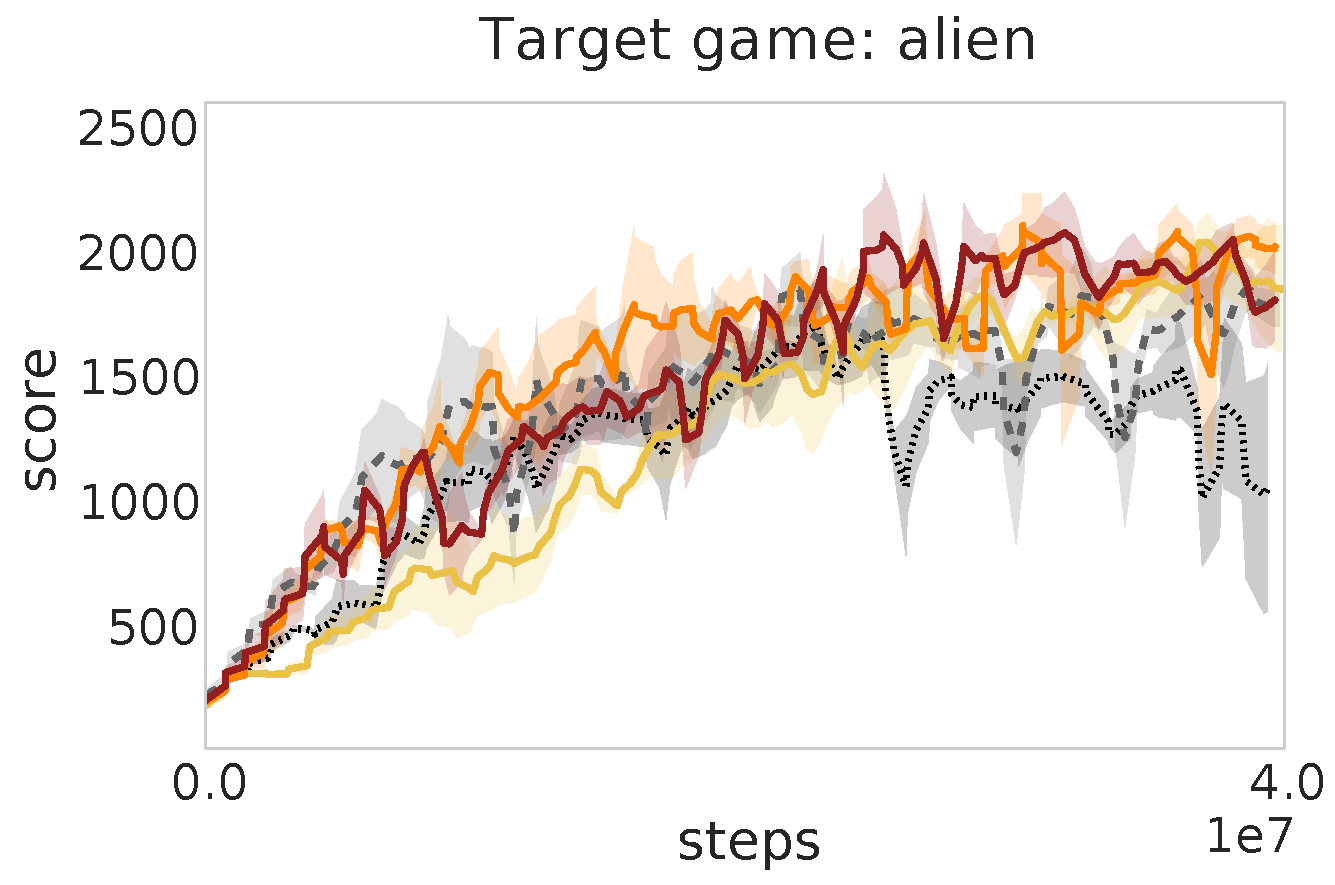
\includegraphics[width=.33\textwidth]{figures/app_plots/mainpaper-nolegend-seaquest_riverraid_pong_to_alien} &
        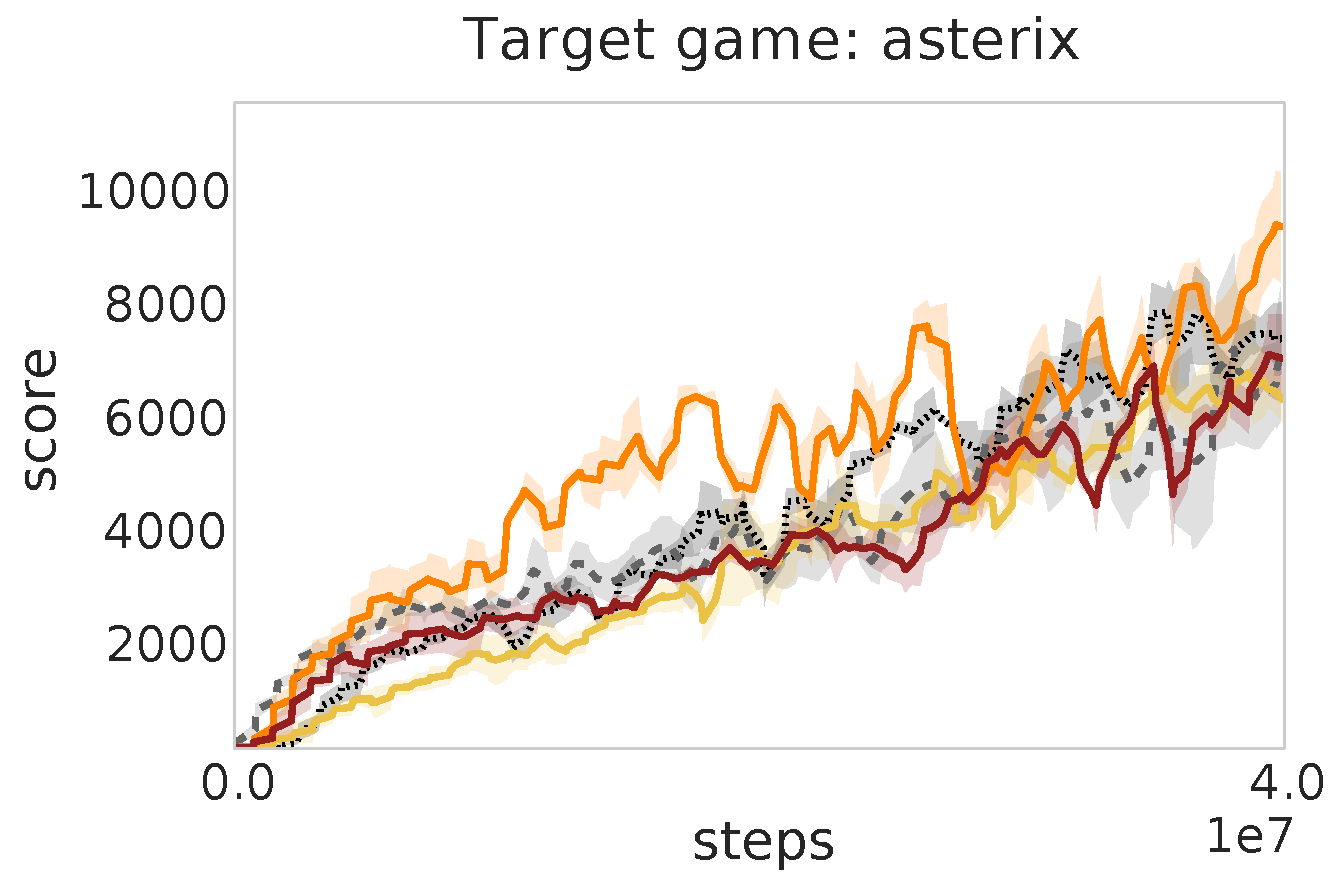
\includegraphics[width=.33\textwidth]{figures/app_plots/mainpaper-nolegend-seaquest_riverraid_pong_to_asterix} &
        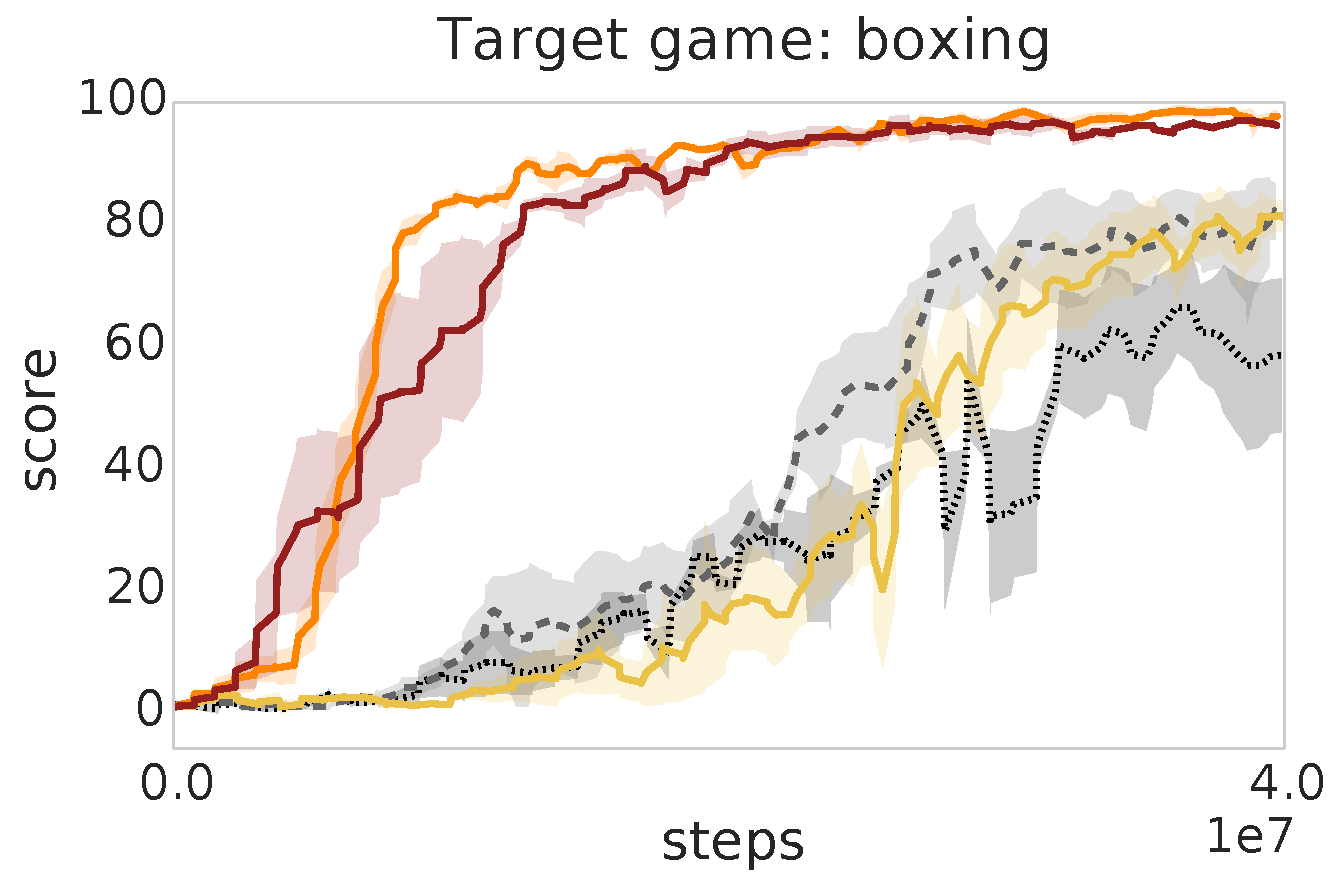
\includegraphics[width=.33\textwidth]{figures/app_plots/mainpaper-nolegend-seaquest_riverraid_pong_to_boxing} \\

        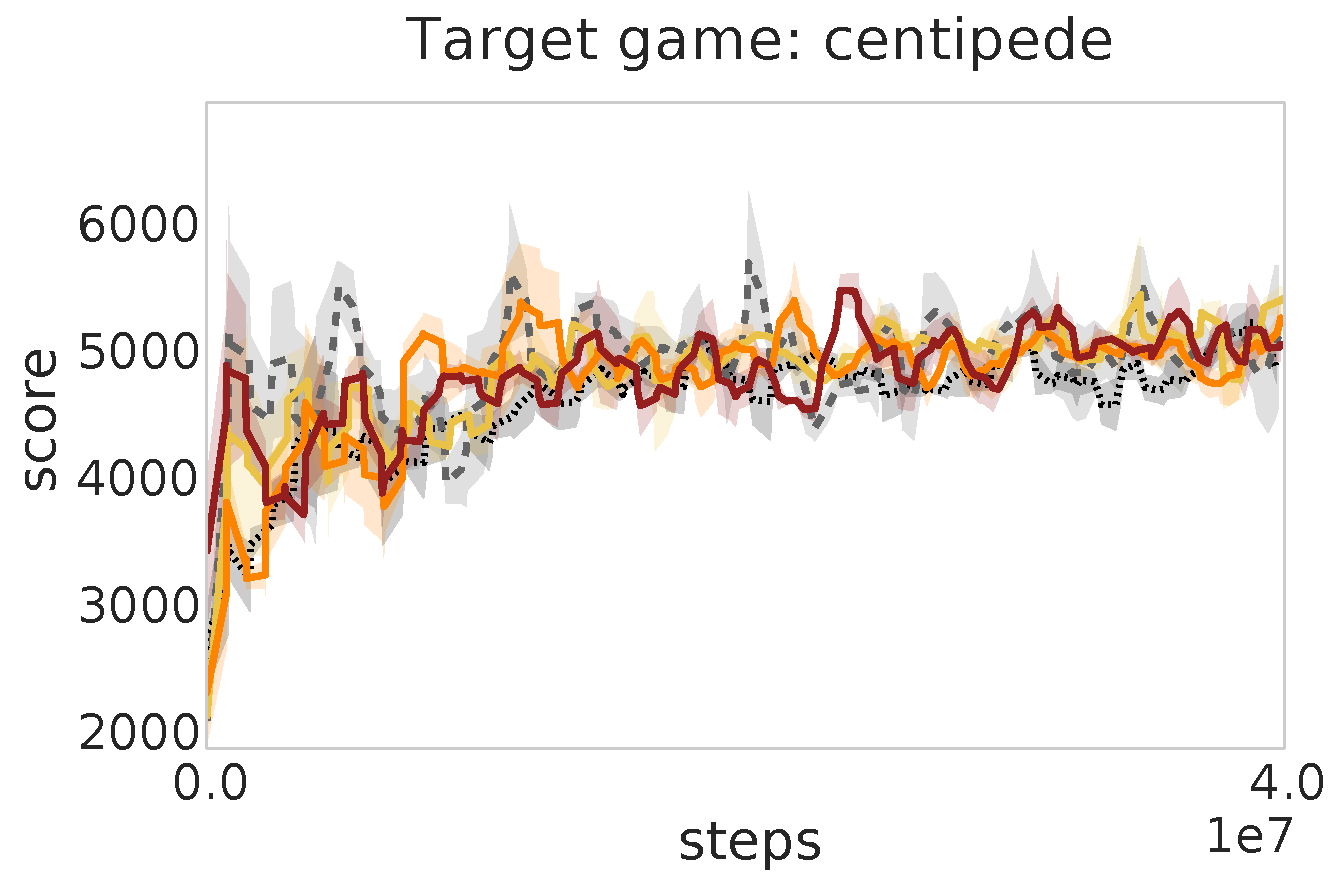
\includegraphics[width=.33\textwidth]{figures/app_plots/mainpaper-nolegend-seaquest_riverraid_pong_to_centipede} &
        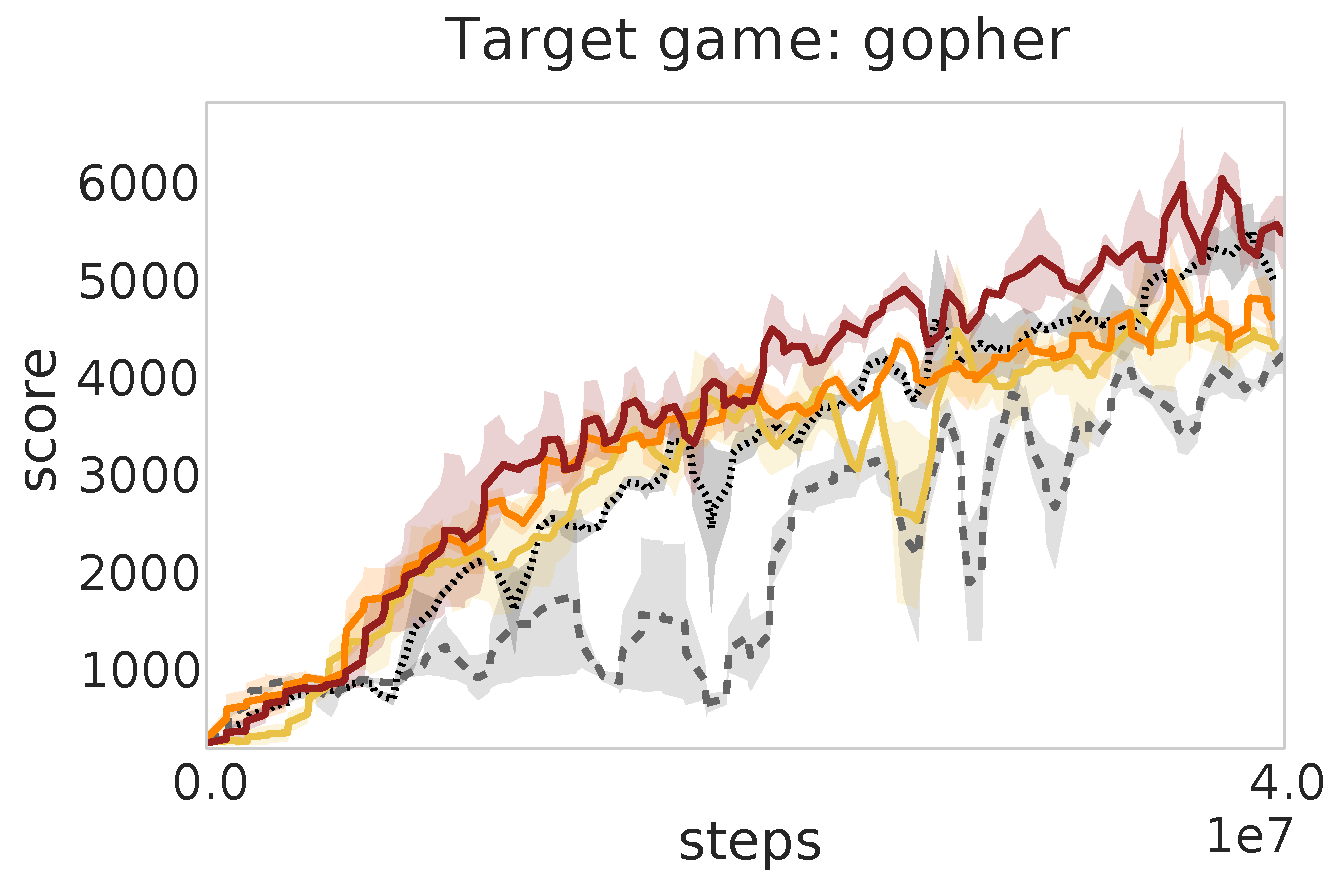
\includegraphics[width=.33\textwidth]{figures/app_plots/mainpaper-nolegend-seaquest_riverraid_pong_to_gopher} &
        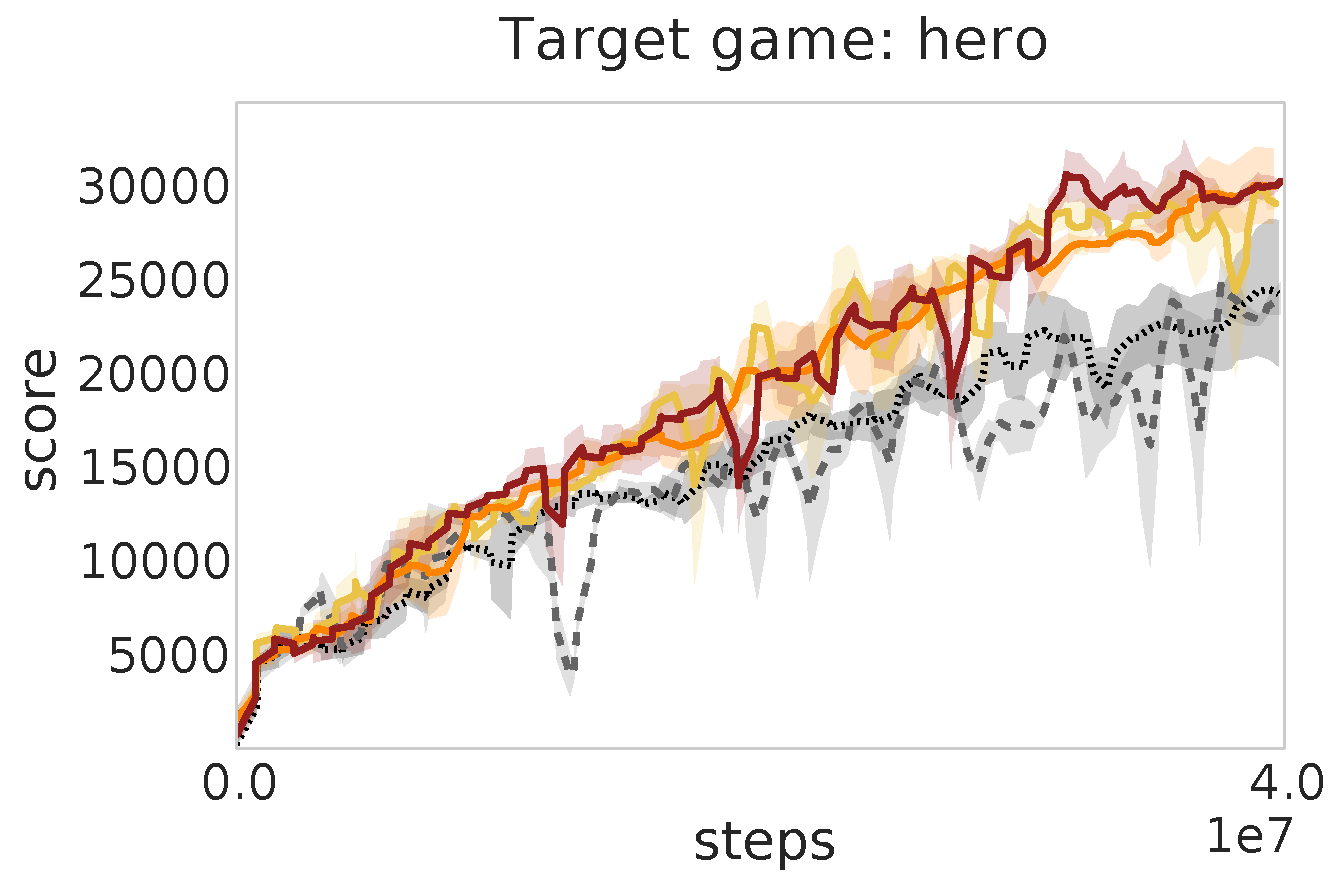
\includegraphics[width=.33\textwidth]{figures/app_plots/mainpaper-nolegend-seaquest_riverraid_pong_to_hero} \\

        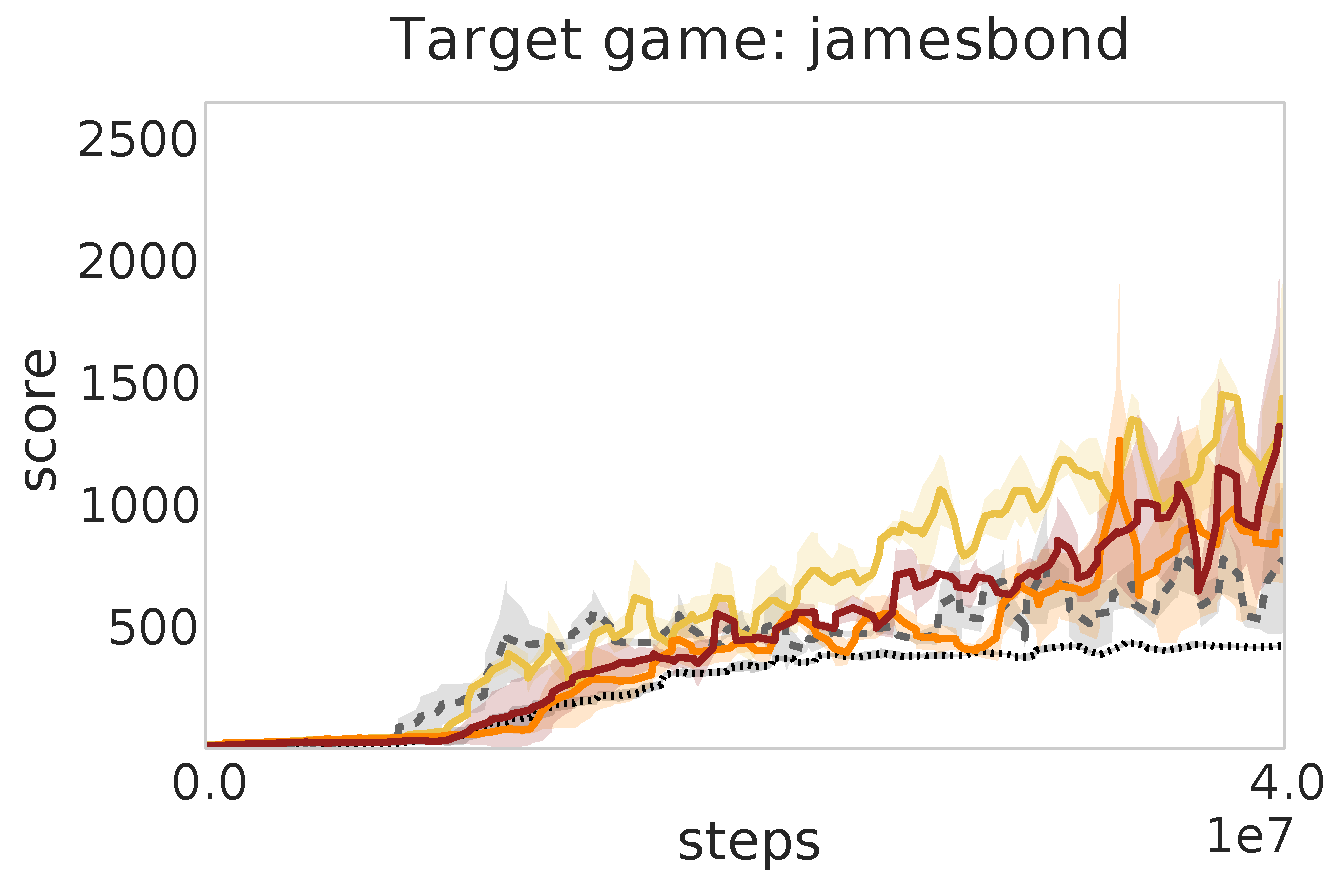
\includegraphics[width=.33\textwidth]{figures/app_plots/mainpaper-nolegend-seaquest_riverraid_pong_to_jamesbond} &
        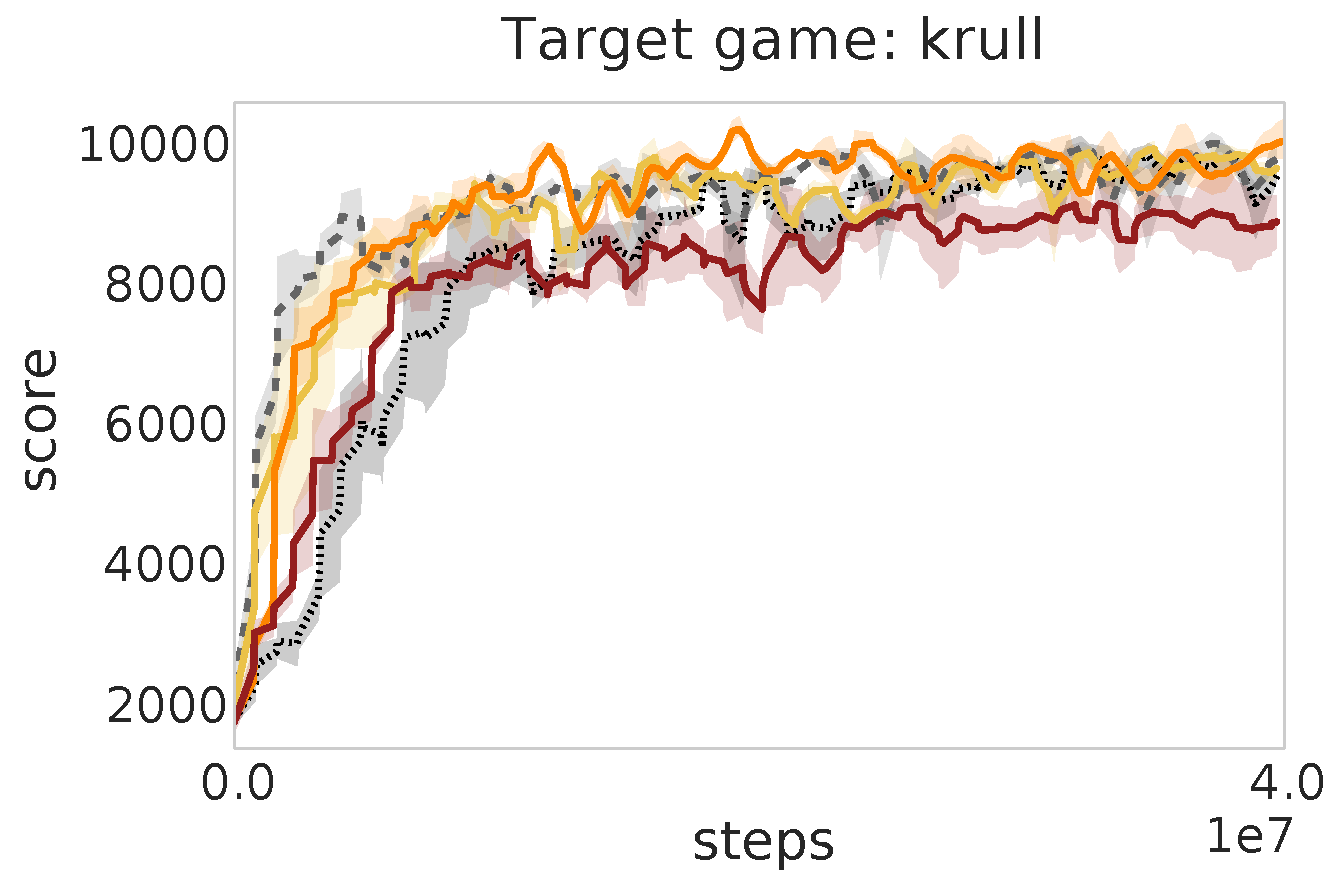
\includegraphics[width=.33\textwidth]{figures/app_plots/mainpaper-nolegend-seaquest_riverraid_pong_to_krull} &
        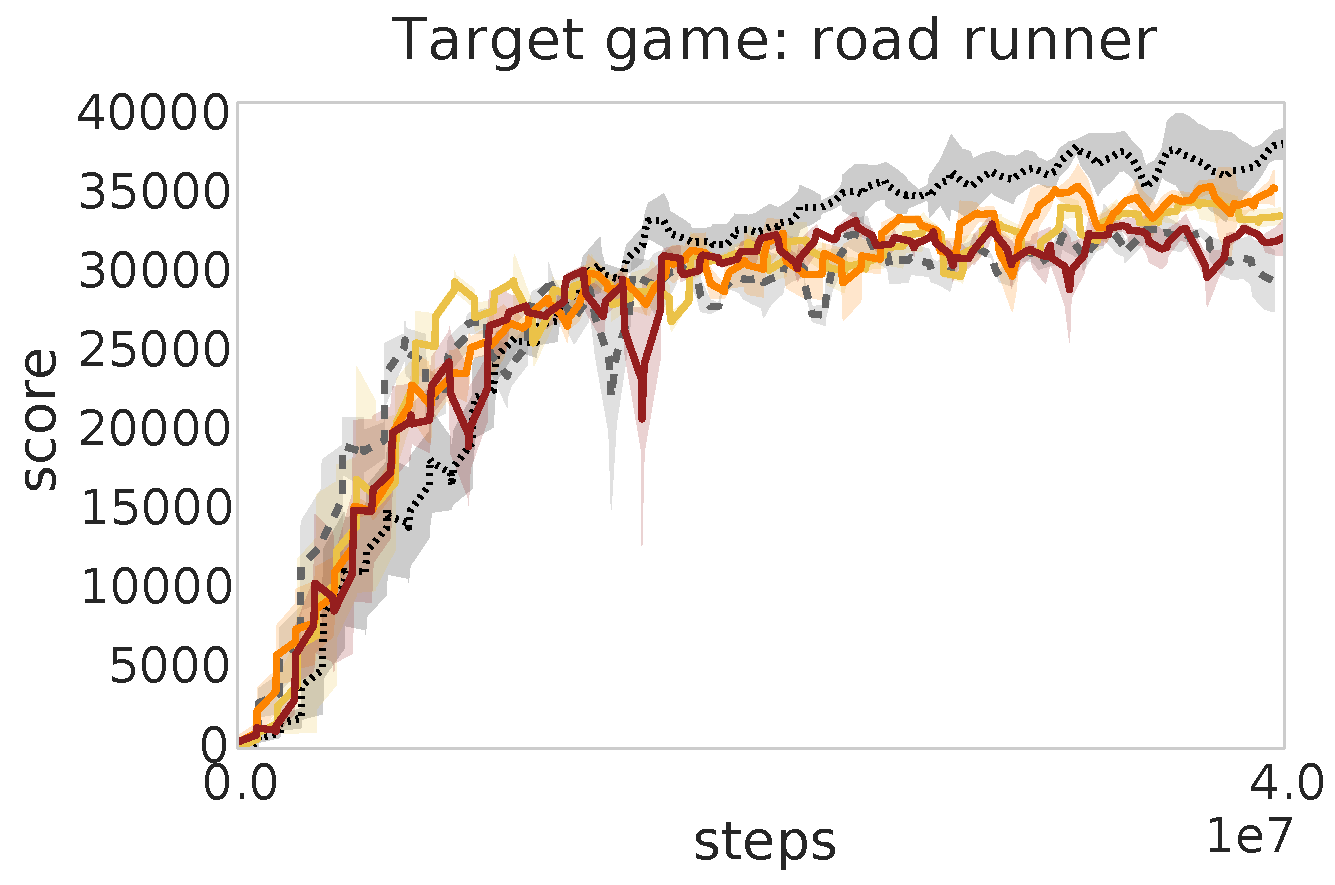
\includegraphics[width=.33\textwidth]{figures/app_plots/mainpaper-nolegend-seaquest_riverraid_pong_to_road_runner} \\

        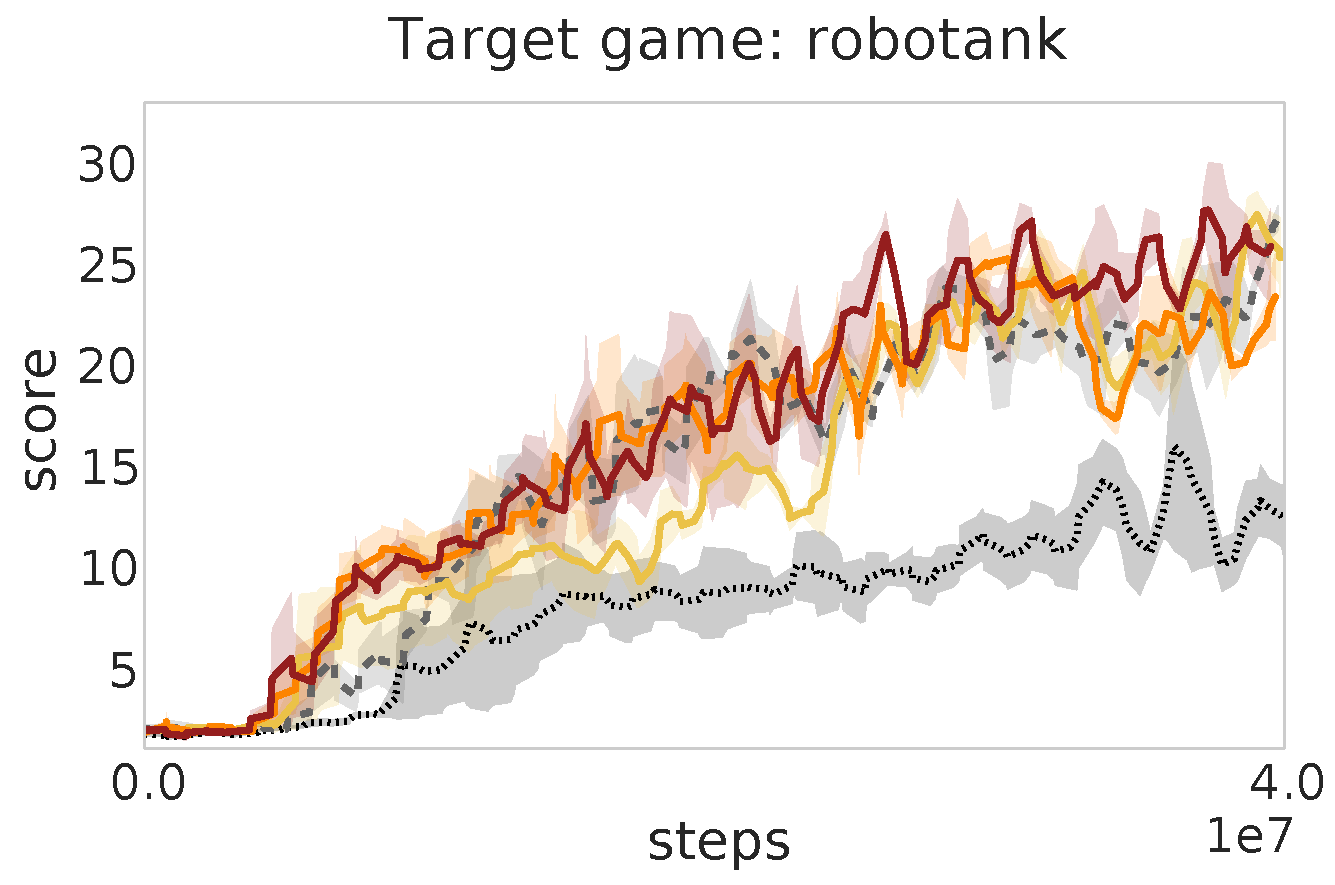
\includegraphics[width=.33\textwidth]{figures/app_plots/mainpaper-nolegend-seaquest_riverraid_pong_to_robotank} &
        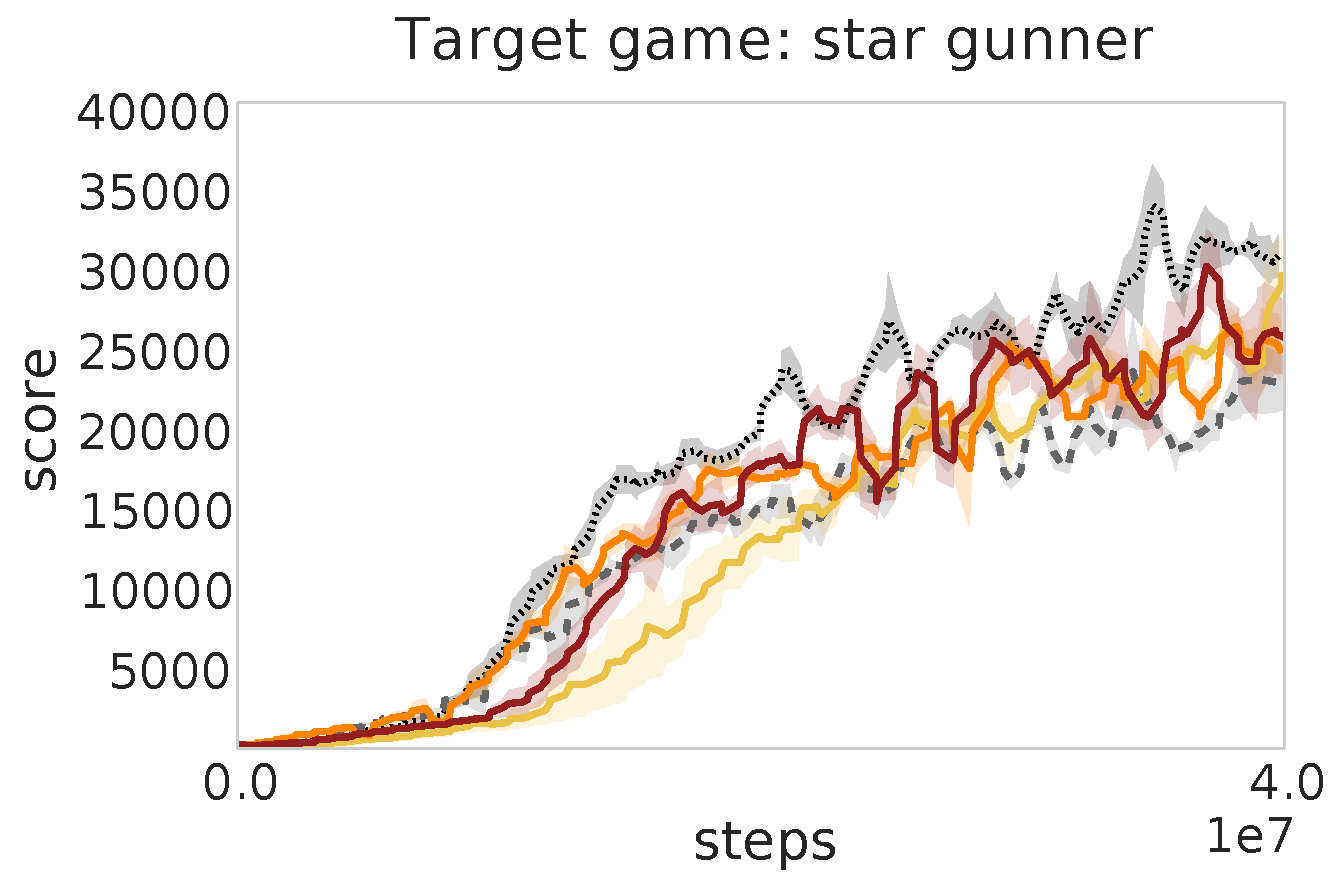
\includegraphics[width=.33\textwidth]{figures/app_plots/mainpaper-nolegend-seaquest_riverraid_pong_to_star_gunner} &
        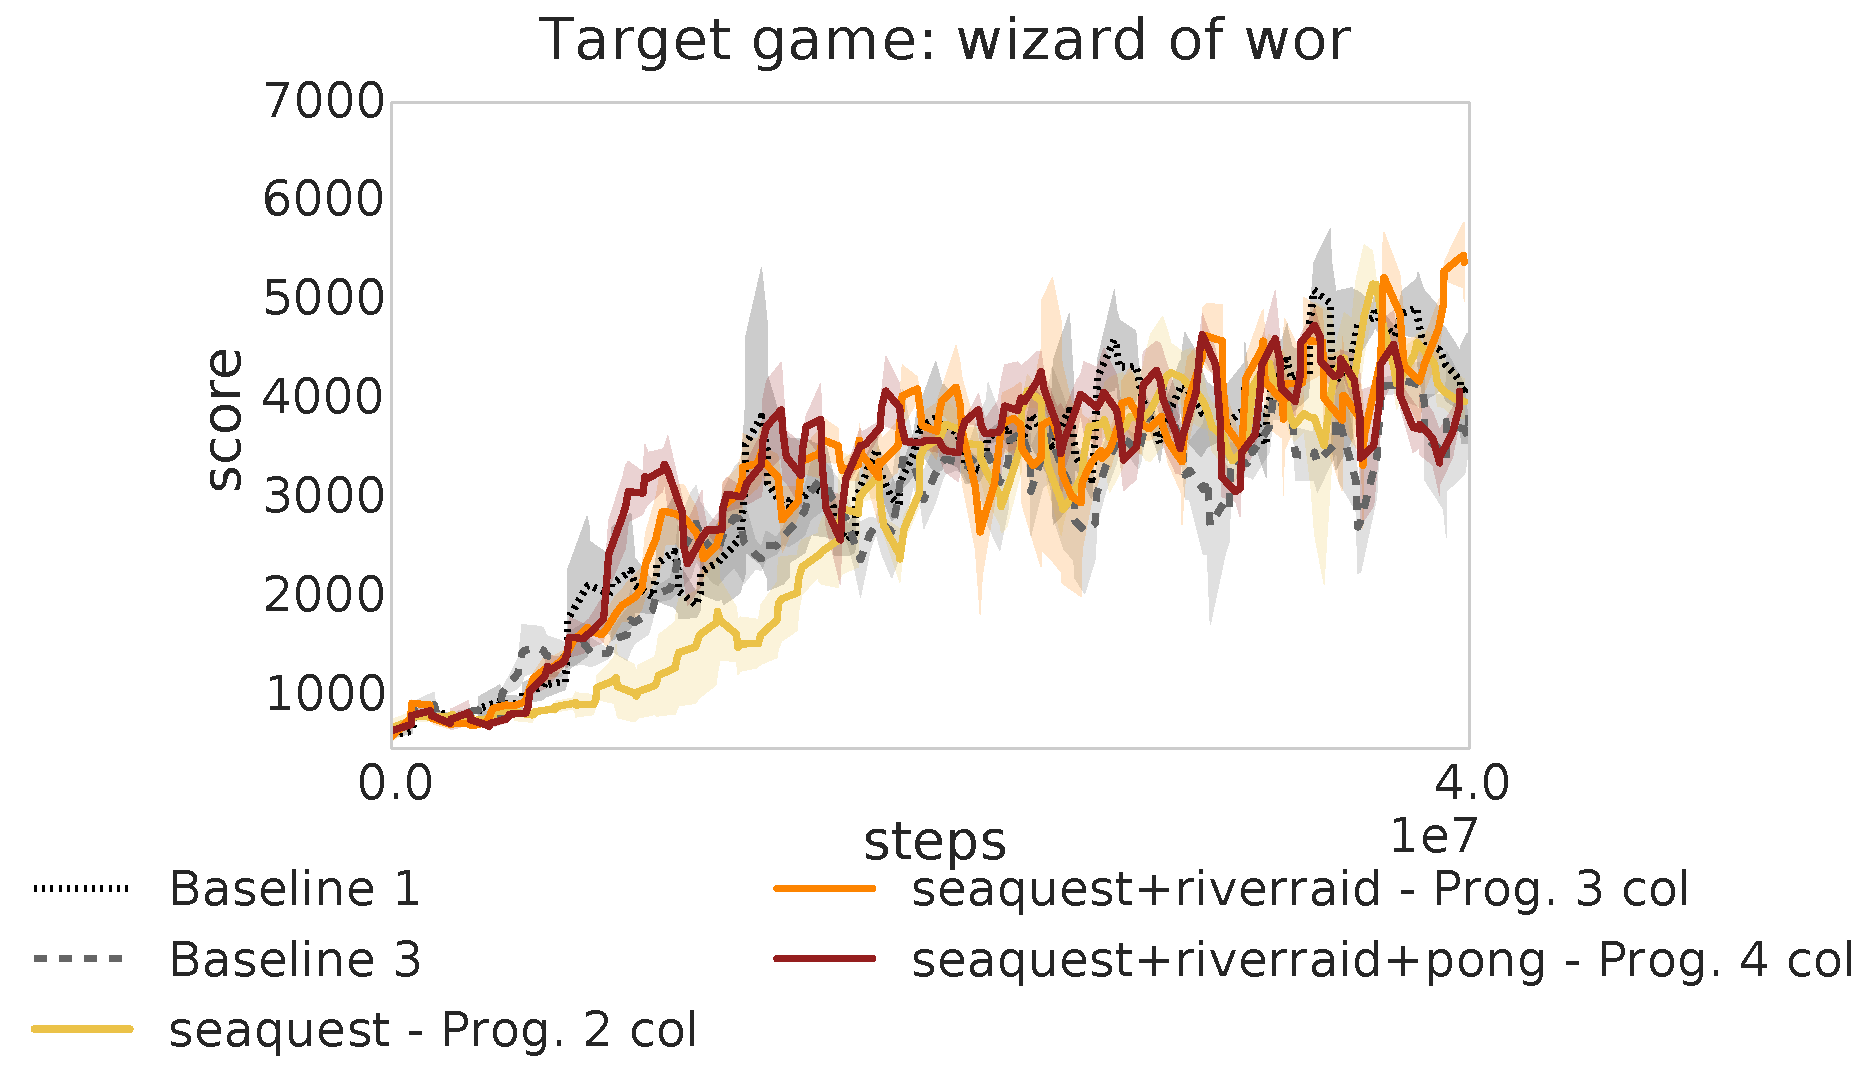
\includegraphics[width=.33\textwidth]{figures/app_plots/mainpaper-legend-seaquest_riverraid_pong_to_wizard_of_wor} \\
    \end{tabular}
    \caption{Training curves for transferring to the \textit{target} games after seeing first Seaquest followed by River Raid and lastly Pong. For the baselines,
    the \textit{source} game used for pretraining is Seaquest.}
    \label{fig:app_plot}
\end{figure}

We can see that overall baseline 3 performs well. However there are situations when having features learned from more previous task actually helps with transfer (e.g. when \textit{target} game is Boxing).

Figure \ref{fig:app_plot_pongs} shows how two-column progressive networks perform as compared to Baseline 3 (gray dashed line), a model pretrained on the \textit{source} game, here standard Pong, and then finetuned on a particular \textit{target} game, and Baseline 1 (black dotted line), where a single column is trained on standard Pong. Figure \ref{fig:app_plot_lab} shows two-column progressive networks and baselines on Labyrinth tasks; the \textit{source} game was Maze Y. 

\begin{figure}
     \begin{tabular}{cccccccc}
	Target: Pong & Target: Black \\
        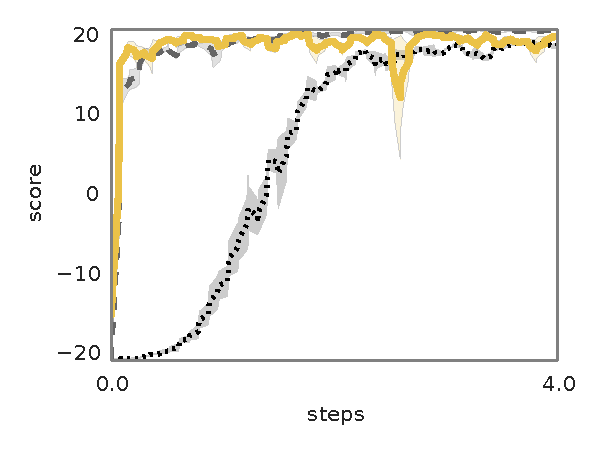
\includegraphics[width=.44\textwidth]{figures/app_plots/pongs/pong/pong} &
        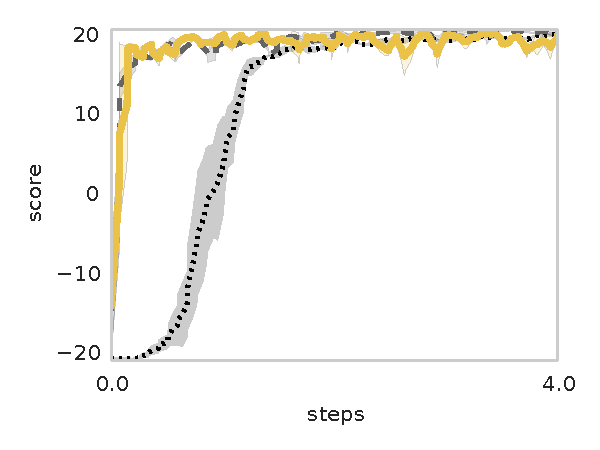
\includegraphics[width=.44\textwidth]{figures/app_plots/pongs/pong/pong_black} \\

	Target: H-flip & Target: HV-flip \\
        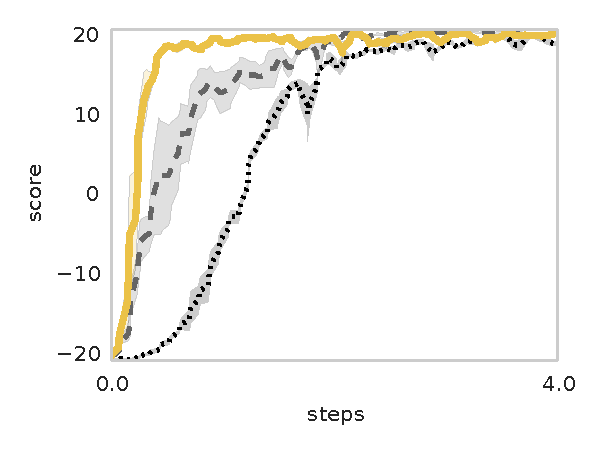
\includegraphics[width=.44\textwidth]{figures/app_plots/pongs/pong/pong_h_flip} &
        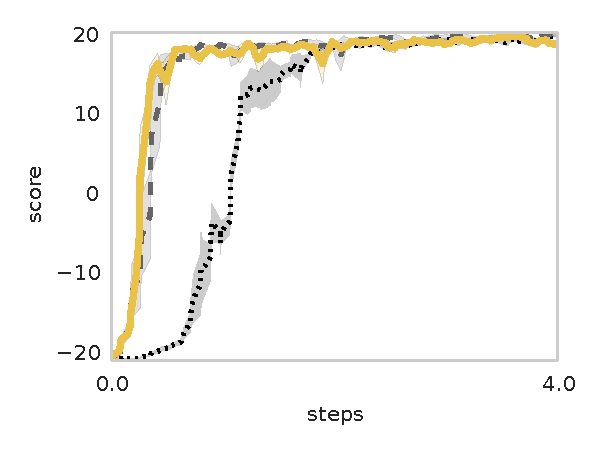
\includegraphics[width=.44\textwidth]{figures/app_plots/pongs/pong/pong_hv_flip} \\

	Target: Noisy & Target: V-flip \\
	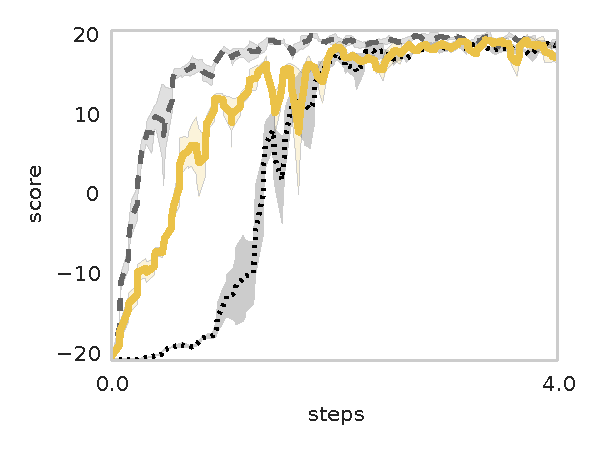
\includegraphics[width=.44\textwidth]{figures/app_plots/pongs/pong/pong_noise} &
        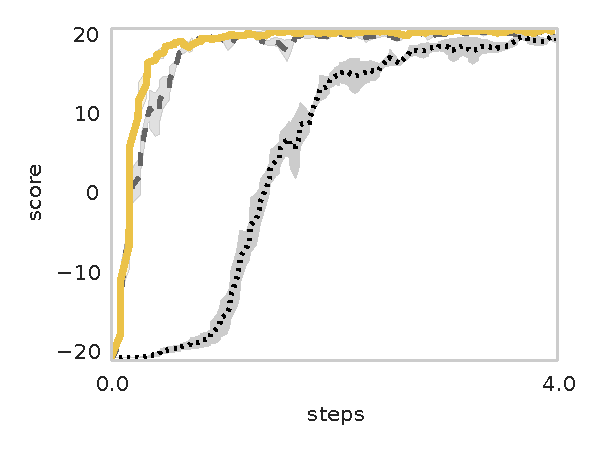
\includegraphics[width=.44\textwidth]{figures/app_plots/pongs/pong/pong_v_flip} \\

	Target: White & Target: Zoom \\
        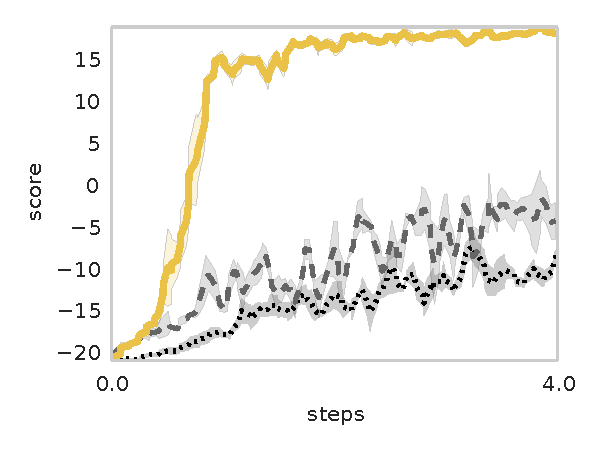
\includegraphics[width=.44\textwidth]{figures/app_plots/pongs/pong/pong_white} &
        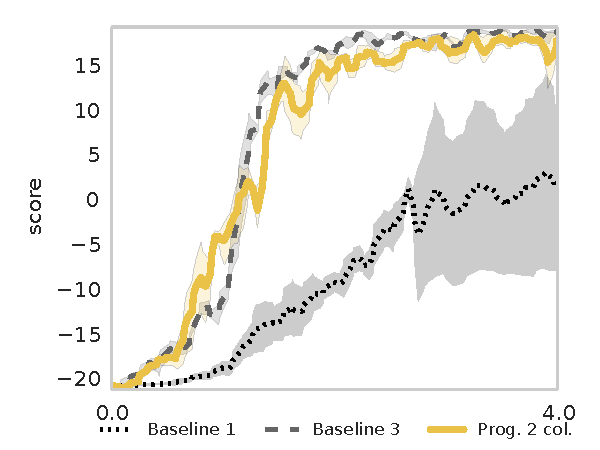
\includegraphics[width=.44\textwidth]{figures/app_plots/pongs_legend/pong/pong_zoom} \\

    \end{tabular}
\caption{Training curves for transferring to 8 \textit{target} games after learning standard Pong first. }
    \label{fig:app_plot_pongs}
\end{figure}

\begin{figure}
     \begin{tabular}{cccccccc}
	Target: Track 1 & Target: Track 2 \\
        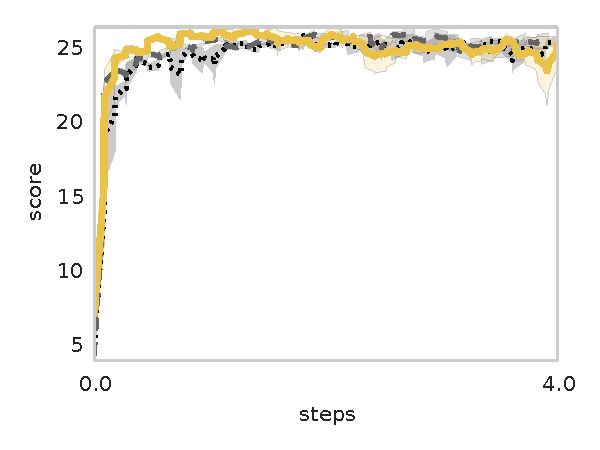
\includegraphics[width=.44\textwidth]{figures/app_plots/lab/smy1/seek_track_01} &
        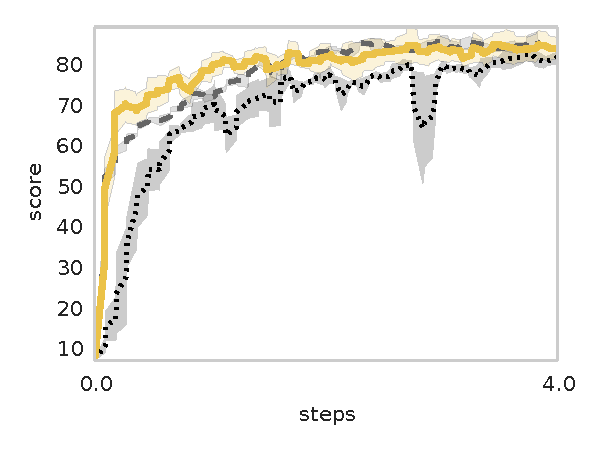
\includegraphics[width=.44\textwidth]{figures/app_plots/lab/smy1/seek_track_02} \\

	Target: Track 3 & Target: Track 4 \\
        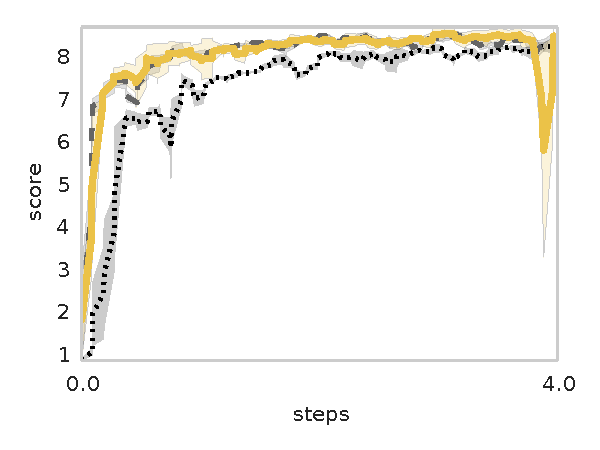
\includegraphics[width=.44\textwidth]{figures/app_plots/lab/smy1/seek_track_03} &
        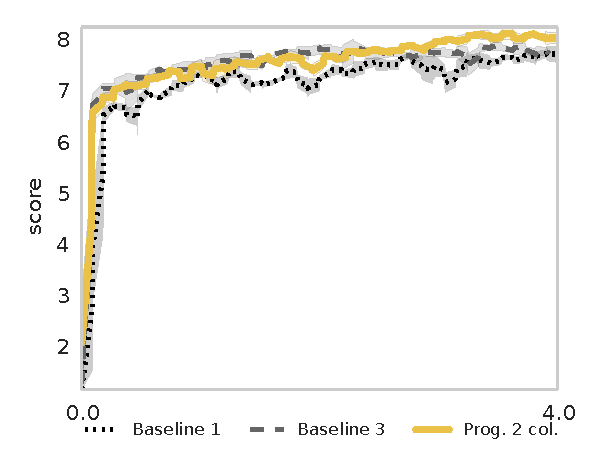
\includegraphics[width=.44\textwidth]{figures/app_plots/lab_legend/smy1/seek_track_04} \\

	Target: Avoid 1 & Target: Avoid 2 \\
        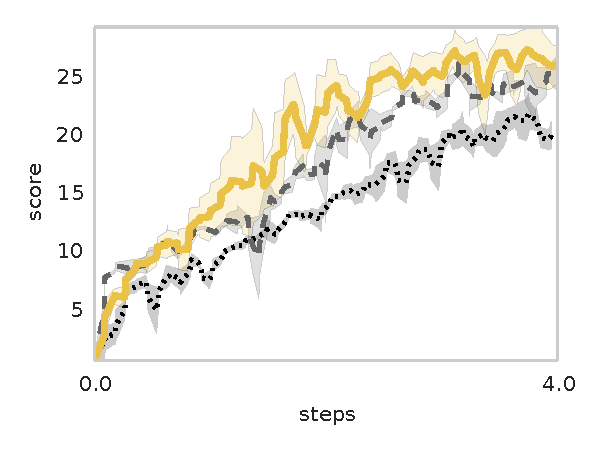
\includegraphics[width=.44\textwidth]{figures/app_plots/lab/smy1/seekavoid_arena_01} &
        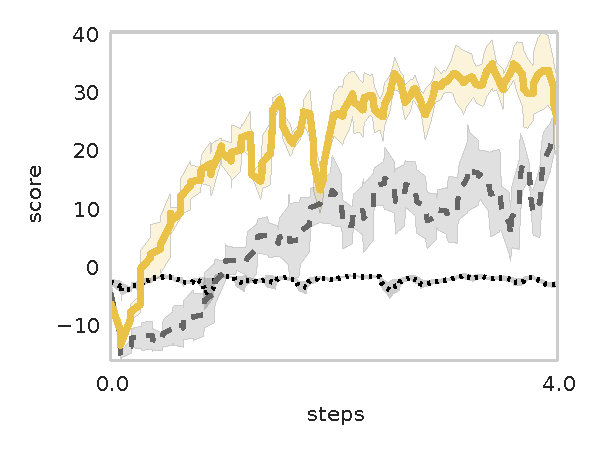
\includegraphics[width=.44\textwidth]{figures/app_plots/lab/smy1/seekavoid_arena_02} \\

	Target: Maze Y & Target: Maze M \\
        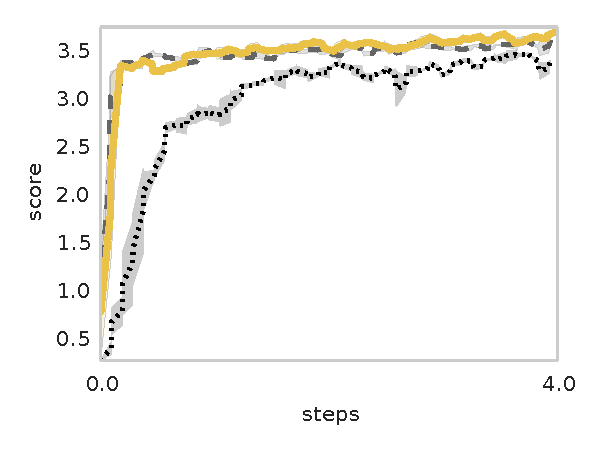
\includegraphics[width=.44\textwidth]{figures/app_plots/lab/smy1/seek_maze_y_01} &
        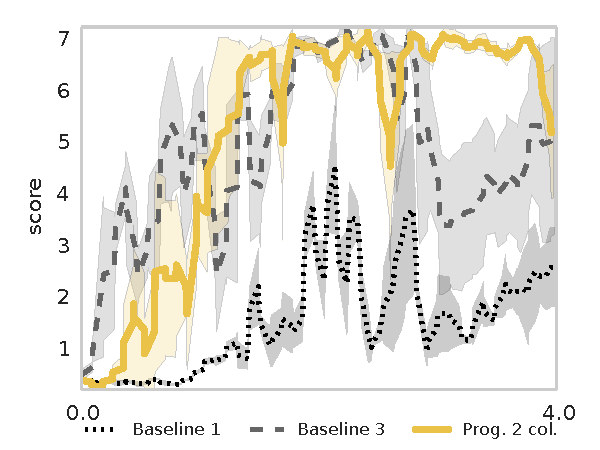
\includegraphics[width=.44\textwidth]{figures/app_plots/lab_legend/smy1/seek_maze_m_01} \\
    \end{tabular}
\caption{Training curves for transferring to 8 \textit{target} games after learning Maze Y first.}
    \label{fig:app_plot_lab}
\end{figure}

